\documentclass[
	spanish,
	9pt,
	xcolor=table,
	handout,
	aspectratio=1610,
	%ignorenonframetext
]{beamer}

\usepackage[spanish]{babel}
\usepackage[
	cursointroductorio,
	fullpagenumbering
]{dunestyle-beamer}
%\usepackage{svg}
%\graphicspath{{./images}}
\usepackage{booktabs}
\usepackage{longtable}

\usepackage[backend=biber,style=numeric, defernumbers=true, sorting=ynt,maxbibnames=4,maxcitenames=4]{biblatex}
\addbibresource{dune-webinar-references.bib}

\title{
	Una introducción a la caja de herramientas DUNE en \texttt{C++}/\texttt{Python} para la solución de modelos matemáticos
}
\subtitle{
	Parte I:
	\lstinline{bash}
}

\author{}
\institute[]
{
	\noindent
	Practique los ejemplos en Gitpod

	\href{https://gitpod.io\#/https://github.com/cpp-review-dune/dune-webinar}{
\includegraphics[width=4.5cm]{open-in-gitpod}}

	\vfill

	\begin{minipage}{0.12\paperwidth}
		Disponible en
	\end{minipage}%
	\hfill%
	\begin{minipage}{0.18\paperwidth}
		\href{https://github.com/cpp-review-dune/dune-webinar}{
\includegraphics[width=1.2cm]{GitHub-Mark-120px-plus}}
	\end{minipage}

	\vfill

	\begin{minipage}{0.26\paperwidth}
		¡Únete al grupo en Telegram!
	\end{minipage}%
	\hfill%
	\begin{minipage}{0.04\paperwidth}
		\href{https://t.me/joinchat/OsfYP1xnFlxjN2Ix}{
\includegraphics[width=1.2cm]{telegram-logo}}
	\end{minipage}

}

\setbeamertemplate{bibliography item}{%
	\ifboolexpr{ test {\ifentrytype{book}} or test {\ifentrytype{mvbook}}
		or test {\ifentrytype{collection}} or test {\ifentrytype{mvcollection}}
		or test {\ifentrytype{reference}} or test {\ifentrytype{mvreference}} }
	{\setbeamertemplate{bibliography item}[book]}
	{\ifentrytype{online}
		{\setbeamertemplate{bibliography item}[online]}
		{\setbeamertemplate{bibliography item}[article]}}%
	\usebeamertemplate{bibliography item}}

\defbibenvironment{bibliography}
{\list{}
	{\settowidth{\labelwidth}{\usebeamertemplate{bibliography item}}%
		\setlength{\leftmargin}{\labelwidth}%
		\setlength{\labelsep}{\biblabelsep}%
		\addtolength{\leftmargin}{\labelsep}%
		\setlength{\itemsep}{\bibitemsep}%
		\setlength{\parsep}{\bibparsep}}}
{\endlist}
{\item}

\begin{document}

{
\usebackgroundtemplate{\centering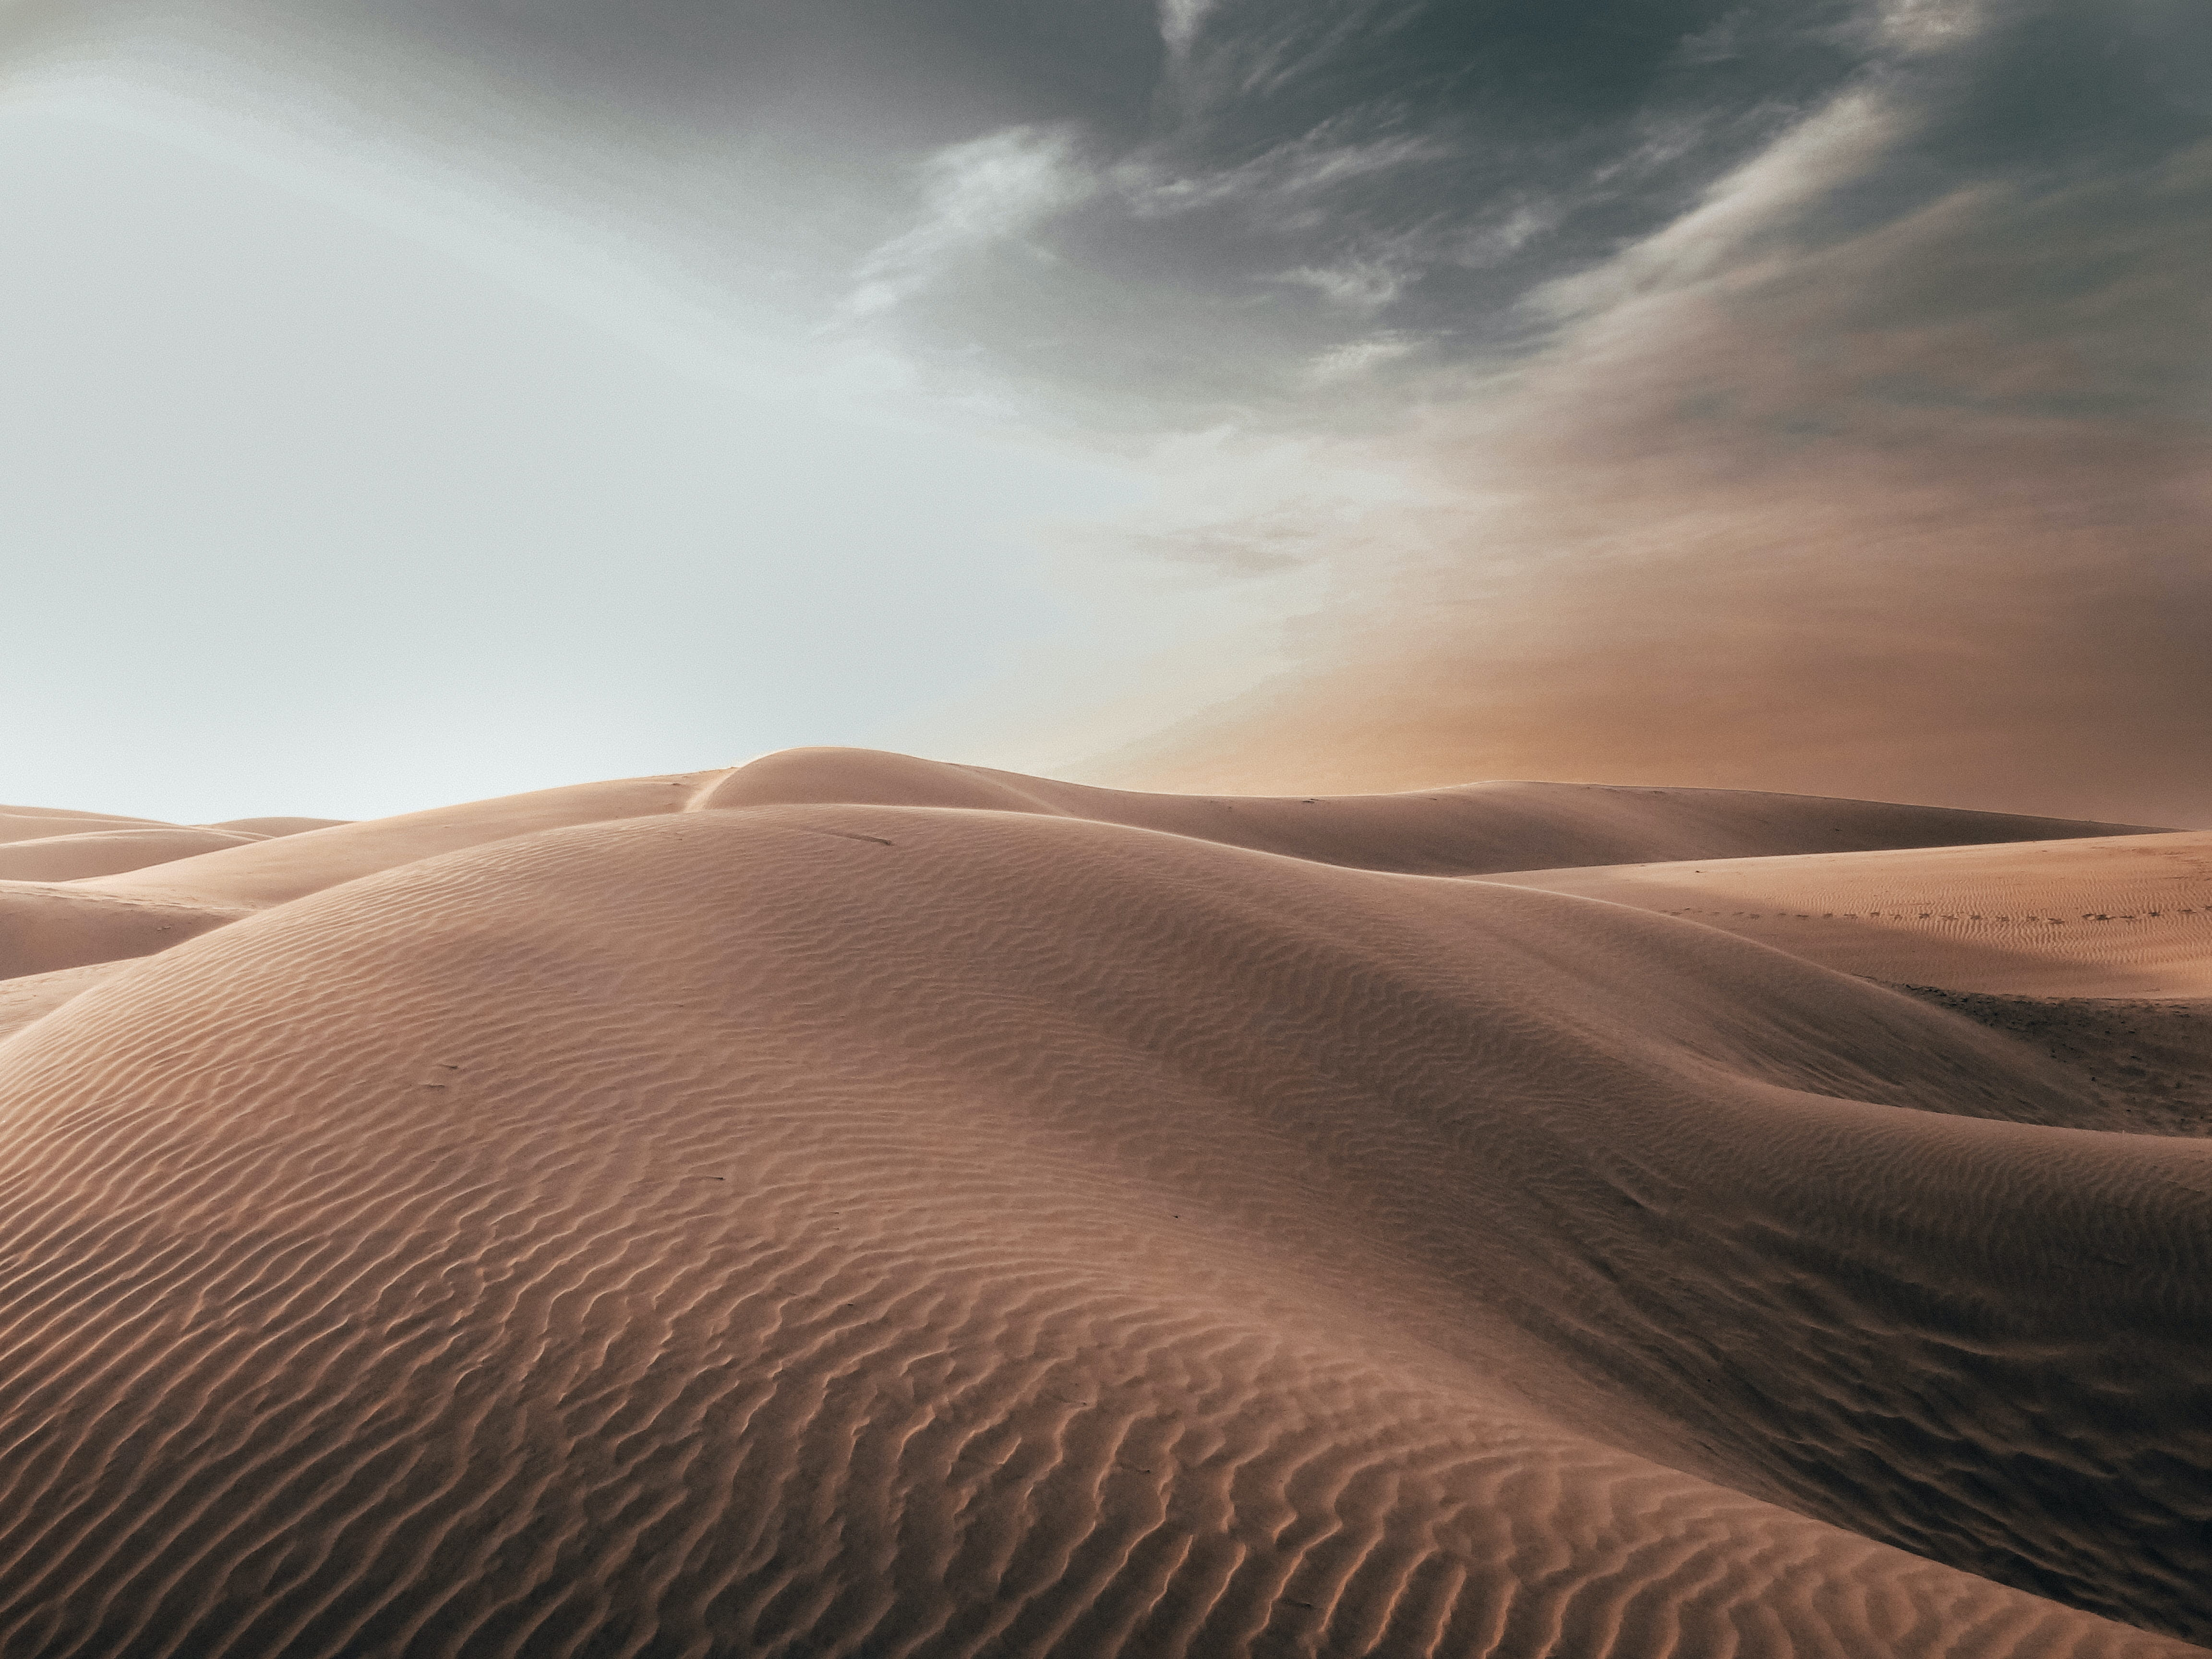
\includegraphics[width=\paperwidth]{duneslides-logo}}
\begin{frame}[plain,noframenumbering]

	\color{c++reviewduneblue}
	
		\begin{flushleft}\bfseries\scshape\huge
		Una introducción a la caja de herramientas Dune en
		C+++/Python para la solución de modelos matemáticos
		\end{flushleft}
	
	\

	\

	\

	\

	\

	\

	\begin{minipage}{0.47\textwidth}
		\begin{figure}[ht!]
		\centering
		
\includegraphics[height=1.5cm]{alfaomega}
		\caption*{\large\bfseries\textcolor{c++reviewduneblue}{Webinar Julio de 2021}}
		\end{figure}
	\end{minipage}
	\begin{minipage}{0.5\textwidth}
		\begin{flushright}\large\bfseries
				Elaborado: John Jairo Leal Gómez\\
				Universidad Nacional de Colombia\\
				Carlos Alonso Aznarán Laos\\
				Universidad Nacional de Ingeniería, Perú
			\end{flushright}
	\end{minipage}

\end{frame}
}

%\frame[plain,noframenumbering]{\titlepage}

\section{Introducción/Presentación del libro}

\begin{frame}
	\frametitle{\secname}
	A.
\end{frame}

\section{DUNE Numerics Project}
\subsection{Introducción}

\begin{frame}
	\frametitle{\secname}
	\framesubtitle{\subsecname}

	\begin{alertblock}{DUNE Numerics}
	Es una caja de herramientas modular desarrollada en C++/Python para la solución numérica de EDPs, utilizando
	métodos basados en mallas, por ejemplo diferencias finitas, elementos finitos o volúmenes finitos.

	\url{https://dune-project.org/about/dune}
	\end{alertblock}

	\begin{figure}[ht!]
		\centering
		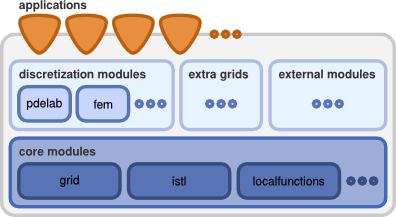
\includegraphics[height=4cm]{dunedesign}
	\end{figure}

\end{frame}

\subsection{El DUNE verso: módulos}
\begin{frame}
	\frametitle{\secname}
	\framesubtitle{\subsecname}

	\begin{figure}[ht!]
	\centering
	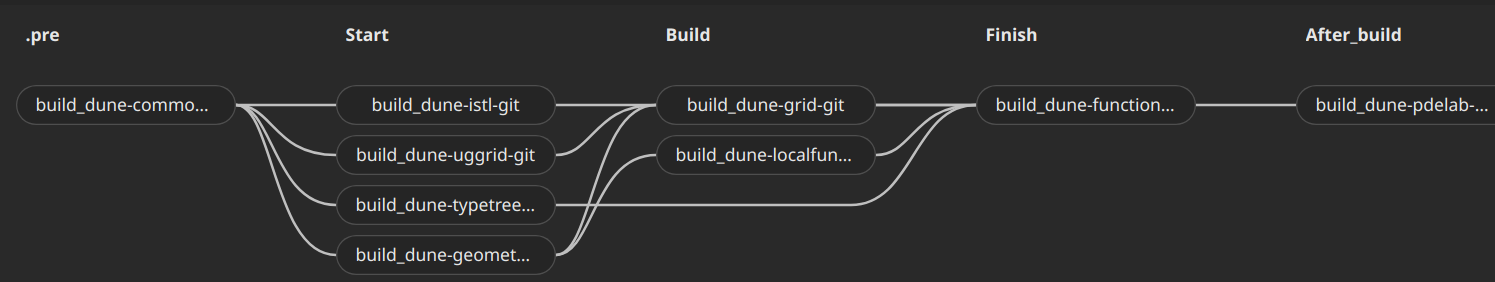
\includegraphics[height=5cm]{dependences.png}
	\end{figure}

	\begin{description}
		\item[dune-common]
			Es minimalista.
			Se usa herramienta pequeñas que sigue la filosofía de UNIX, de modo que tengas una base muy pequeña que deje configurar la máquina de manera más cómoda para el usuario.
		\item[dune-geometry]
			Mantener la paquetería lo más actualizada posible sin sacrificar la estabilidad. Cuenta con los compiladores más actuales de \lstinline{gcc}, \lstinline{lualatex}, \lstinline{go}, etc.
	\end{description}

\end{frame}

{
\usebackgroundtemplate{\centering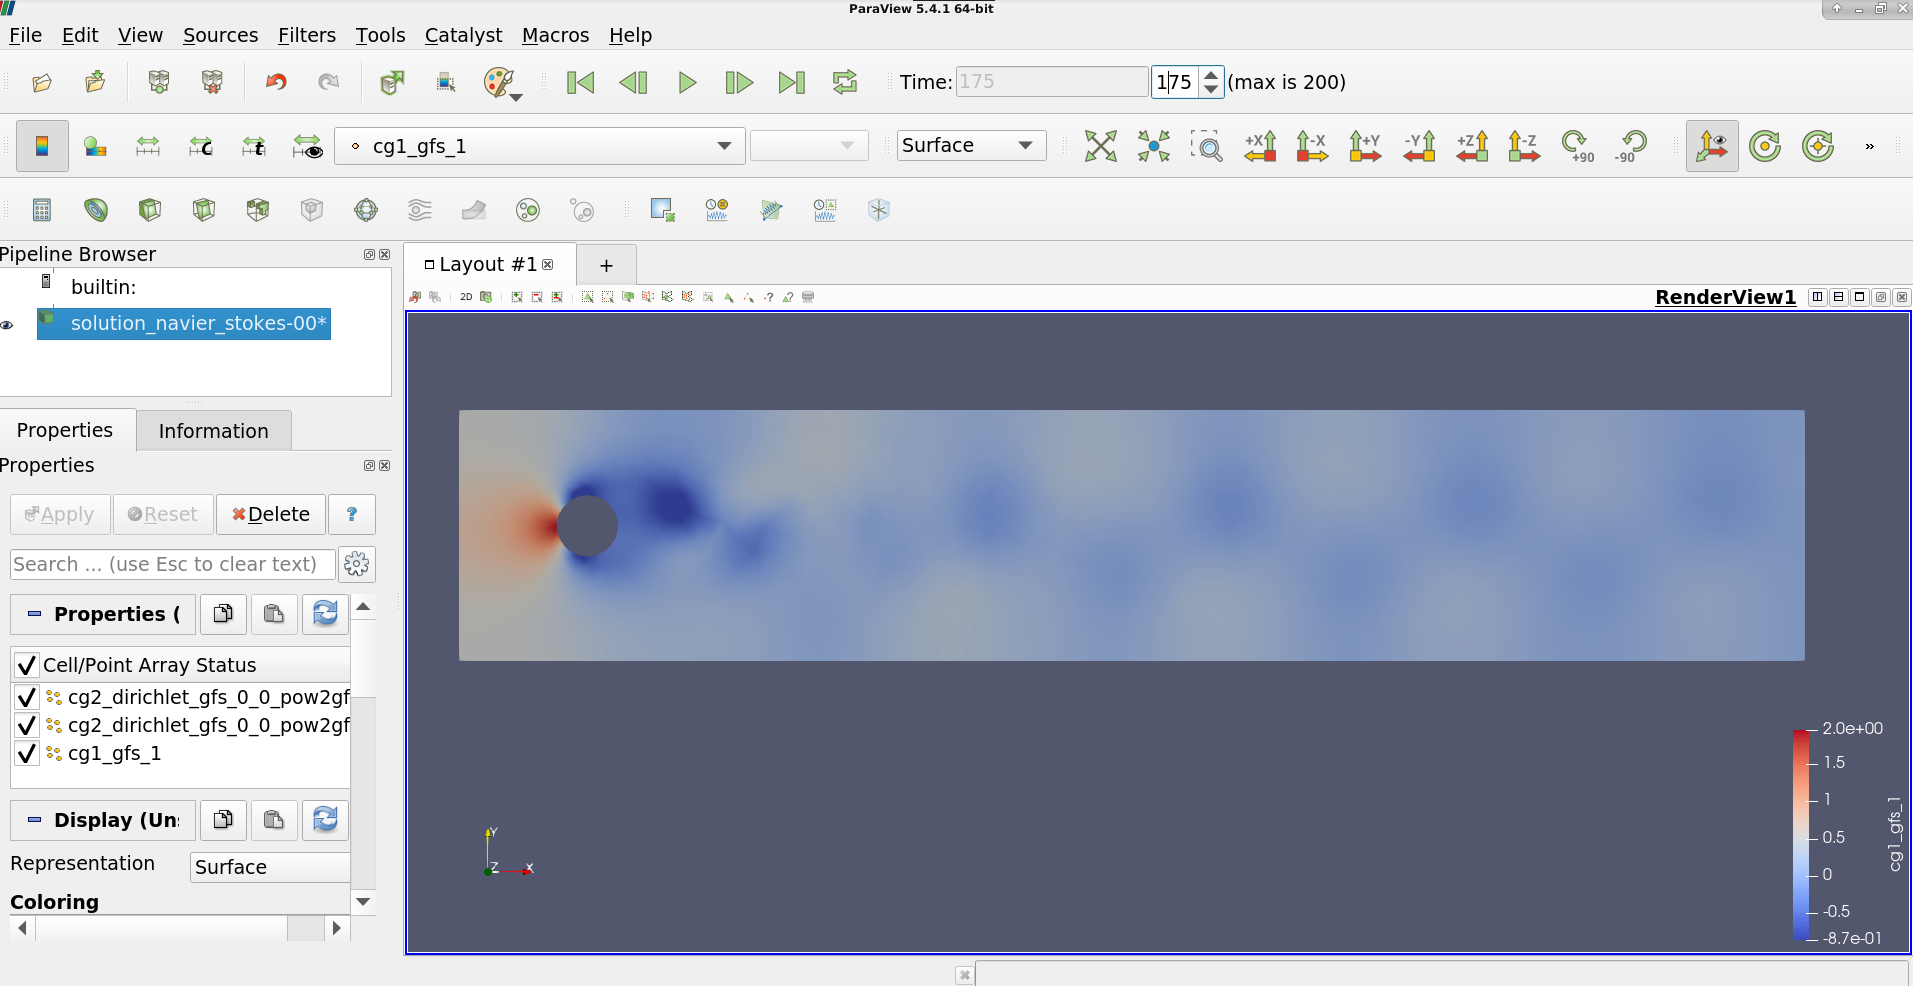
\includegraphics[width=\paperwidth]{tutorial-9}}
\begin{frame}[plain]
\end{frame}
}

\begin{frame}
	\frametitle{\secname}
	\framesubtitle{\subsecname}

	
\end{frame}

\begin{frame}
	
\end{frame}

\begin{frame}
	
\end{frame}

%\begin{frame}[fragile]
%	\begin{lstlisting}
%    gitpod ~/dune-basics $ cd
%  \end{lstlisting}
%\end{frame}


\begin{frame}
	\frametitle{El comando \lstinline{duneproject}}

\end{frame}

\begin{frame}\transblindsvertical
	\frametitle{Referencias}
	%------------------------------------------------------------ 1
	\only<1>{
		\begin{itemize}
			\item Libros
			      \nocite{*}
			      \printbibliography[heading=none,keyword=book]
		\end{itemize}
	}
	%------------------------------------------------------------ 2
	\only<2>{
		\begin{itemize}
			\item Artículos
			      \printbibliography[heading=none,keyword=paper]
		\end{itemize}
	}
	%------------------------------------------------------------ 3
	\only<3>{
		\begin{itemize}
			\item Sitios web
			      \printbibliography[heading=none,keyword=online]
		\end{itemize}
	}
\end{frame}

\end{document}